\chapter{Mensageiros químicos e transdução de sinais}\label{ch:b2:cell-signalling}

Uma única molécula de adrenalina que chega à superfície de uma célula
do fígado nunca entra nela. Ela se liga a uma proteína do lado de fora,
muda a forma dessa proteína e, em um segundo, a célula produziu dez mil
moléculas de um \omterm{prop:b2:cell-signalling:gpcr}{segundo mensageiro}, ativou cem mil moléculas de enzima
e começou a liberar um milhão de moléculas de glicose --- uma cadeia de
amplificações de um milhão de vezes, iniciada por um sinal que ficou do
lado de fora da porta. Este capítulo trata dos mensageiros que as
células enviam umas às outras e de como uma célula converte uma
mensagem em sua superfície numa mudança de sua química, de seus genes
ou de sua forma: os receptores, os \omterm{prop:b2:cell-signalling:gpcr}{segundos mensageiros}, as cascatas de
quinases e os dois modelos --- a sinalização rápida e por fios dos
nervos e a sinalização lenta e difundida dos \omterm{def:b2:cell-signalling:kinds}{hormônios} --- cujo
contraste atravessa o resto deste livro.

\section{Os mensageiros}

\begin{definition}[Tipos de sinalização química]\label{def:b2:cell-signalling:kinds}
\index{hormônio}\index{sinalização endócrina}\index{sinalização parácrina}\index{neurotransmissor}
Uma célula sinaliza a outra por meio de uma molécula secretada, um
\emph{mensageiro} ou \emph{ligante}, que se liga a um \emph{receptor}
na célula-alvo ou dentro dela. Pelo alcance: a sinalização
\emph{endócrina}, na qual um \emph{hormônio} é liberado no \omterm{def:b2:blood-circulation:blood}{sangue} por
uma glândula e chega a todas as células do corpo, agindo apenas sobre
as que têm o receptor, ao longo de minutos a horas (insulina, cortisol,
adrenalina, tiroxina); a sinalização \emph{parácrina}, na qual o
mensageiro se difunde até as células vizinhas, a menos de um milímetro,
e é destruído no caminho (fatores de crescimento, histamina,
prostaglandinas, os morfógenos do \cref{ch:b2:vertebrate-development}); a \emph{autócrina}, em que
a célula sinaliza a si mesma; e a \emph{sináptica}, na qual um neurônio
libera um \emph{neurotransmissor} através de um espaço de
\qty{20}{nm} sobre uma única célula-alvo, em um milissegundo
(\cref{ch:b2:neurons-synapses}). Pela química: os mensageiros \emph{hidrossolúveis} ---
derivados de aminoácidos, como a adrenalina, peptídeos e proteínas,
como a insulina --- não conseguem atravessar a membrana e agem sobre
receptores de superfície; os mensageiros \emph{lipossolúveis} --- os
esteroides (cortisol, estradiol, testosterona), a tiroxina, o ácido
retinoico, o óxido nítrico --- a atravessam e agem sobre receptores
internos. Os sistemas endócrino e nervoso são as duas maneiras pelas
quais um corpo de $10^{13}$ células se coordena: um transmite
lentamente para todos, o outro liga rapidamente por fio a alguém.
\end{definition}

\begin{omfigure}
\begin{tikzpicture}[every node/.style={font=\scriptsize}, >=stealth]
  % endocrine
  \begin{scope}
    \draw[thick, fill=omProp!25] (0,1.6) circle (0.35); \node[above] at (0,2.0) {glândula};
    \draw[very thick, omThm!60] (-0.5,0.6) -- (4.5,0.6); \draw[very thick, omThm!60] (-0.5,0.2) -- (4.5,0.2); \node[omThm!70!black] at (2,0.4) {sangue};
    \foreach \x in {0.6,1.5,2.4,3.3} \fill[omProp] (\x,0.4) circle (0.05);
    \draw[->, omProp] (0,1.25) -- (0,0.65);
    \draw[thick, fill=omDef!20] (3.8,-0.8) circle (0.35); \node[below, align=center] at (3.8,-1.2) {célula-alvo\\com receptor};
    \draw[->, omProp] (3.8,0.15) -- (3.8,-0.4);
    \draw[thick, fill=gray!20] (1.0,-0.8) circle (0.35); \node[below, align=center] at (1.0,-1.2) {sem receptor:\\ignora-o};
    \node[align=center] at (2.2,-2.4) {endócrina: hormônio no sangue,\\corpo inteiro, de minutos a horas};
  \end{scope}
  % paracrine
  \begin{scope}[xshift=6.6cm]
    \draw[thick, fill=omProp!25] (0.8,0.6) circle (0.35);
    \foreach \a in {0,45,...,315} \fill[omProp] (0.8,0.6) ++(\a:0.6) circle (0.04);
    \draw[thick, fill=omDef!20] (1.9,0.9) circle (0.3); \draw[thick, fill=omDef!20] (1.7,-0.2) circle (0.3); \draw[thick, fill=omDef!20] (-0.2,0.0) circle (0.3);
    \node[align=center] at (0.8,-2.4) {parácrina: difunde-se\\até as vizinhas, destruída\\em um milímetro};
  \end{scope}
  % synaptic
  \begin{scope}[xshift=11.6cm]
    \draw[very thick, omDef] (0,1.8) -- (0,0.5); \draw[thick, fill=omDef!25] (0,0.3) circle (0.25);
    \draw[thick, fill=omExo!30] (0,-0.5) circle (0.3);
    \foreach \x in {-0.08,0,0.08} \fill[omProp] (\x,-0.05) circle (0.03);
    \node[align=center] at (0.2,-2.4) {sináptica: um único alvo,\\\qty{20}{nm},\\um milissegundo};
  \end{scope}
\end{tikzpicture}

{\small Três alcances da sinalização química: um \omterm{def:b2:cell-signalling:kinds}{hormônio} difundido pelo
\omterm{def:b2:blood-circulation:blood}{sangue} a todas as células que têm seu receptor; um fator parácrino que
chega às vizinhas; um \omterm{def:b2:cell-signalling:kinds}{neurotransmissor} entregue através de uma sinapse
a uma única célula.}
\end{omfigure}

\begin{theorem}[A ocupação dos receptores]\label{thm:b2:cell-signalling:occupancy}
\index{constante de dissociação}\index{ocupação dos receptores}
Um receptor $R$ se liga de modo reversível a seu ligante $L$, $R + L
\rightleftharpoons RL$, com uma \emph{\omterm{thm:b2:cell-signalling:occupancy}{constante de dissociação}} $K_d =
[R][L]/[RL]$. No equilíbrio, a fração de receptores ocupados é
\[
\theta = \frac{[RL]}{[R]_{\text{tot}}} = \frac{[L]}{K_d + [L]},
\]
a mesma hipérbole da saturação de uma enzima. $K_d$ é a concentração na
qual metade dos receptores está ocupada e mede a \emph{afinidade}:
quanto menor, mais forte. Os receptores hormonais têm
$K_d$ na faixa de nanomolar a picomolar, ajustada às concentrações em
que os \omterm{def:b2:cell-signalling:kinds}{hormônios} circulam ($10^{-12}$ a
$10^{-9}$ mol/L): com $[L] = K_d/10$, um décimo está ocupado; com
$10K_d$, nove décimos. Uma célula não consegue responder a um \omterm{def:b2:cell-signalling:kinds}{hormônio}
para o qual não tem receptores, e ajusta sua sensibilidade mudando o
número de receptores, ou --- como no \cref{ch:b2:reproductive-hormones} --- retirando-os quando o
\omterm{def:b2:cell-signalling:kinds}{hormônio} está constantemente presente.
\end{theorem}
\begin{proof}
Com $[R] = [R]_{\text{tot}} - [RL]$, $K_d = ([R]_{\text{tot}} -
[RL])[L]/[RL]$, de modo que $[RL](K_d + [L]) = [R]_{\text{tot}}[L]$, que
é a fórmula. É a expressão de Michaelis--Menten do volume do Ano 1 sem
a etapa catalítica.
\end{proof}

\begin{omfigure}
\begin{tikzpicture}
\begin{axis}[
  width=0.68\linewidth, height=5.2cm,
  axis x line=bottom, axis y line=left,
  xmode=log, xmin=0.01, xmax=100, ymin=0, ymax=1.1,
  xlabel={concentração do ligante (em unidades de $K_d$)}, ylabel={fração de receptores ocupados},
  xlabel style={font=\small, at={(axis description cs:0.5,-0.13)}, anchor=north},
  ylabel style={font=\small},
  tick label style={font=\small}, xtick={0.01,0.1,1,10,100}, ytick={0,0.5,1},
  clip=false,
]
\addplot[very thick, omDef, domain=0.01:100, samples=100] {x/(1+x)};
\draw[dashed, gray] (axis cs:1,0) -- (axis cs:1,0.5) -- (axis cs:0.01,0.5);
\node[font=\scriptsize, anchor=north west] at (axis cs:1.1,0.48) {$[L] = K_d$: metade ocupada};
\node[font=\scriptsize, anchor=south east] at (axis cs:0.1,0.1) {10\% em $K_d/10$};
\node[font=\scriptsize, anchor=north west] at (axis cs:10,0.92) {90\% em $10\,K_d$};
\end{axis}
\end{tikzpicture}

{\small \omterm{thm:b2:cell-signalling:occupancy}{Ocupação dos receptores} em função da concentração do ligante,
em escala logarítmica: a resposta de uma célula vai de um décimo a nove
décimos numa faixa de concentração de cem vezes centrada em $K_d$.}
\end{omfigure}

\section{Os receptores de superfície}

\begin{proposition}[Os receptores acoplados à proteína G e o AMP cíclico]\label{prop:b2:cell-signalling:gpcr}
\index{proteína G}\index{receptor acoplado à proteína G}\index{AMP cíclico}\index{segundo mensageiro}\index{proteína quinase A}
A maior família de receptores --- cerca de \num{800} genes no ser
humano, para \omterm{def:b2:cell-signalling:kinds}{hormônios}, \omterm{def:b2:cell-signalling:kinds}{neurotransmissores}, odores, luz --- é formada
por proteínas que atravessam a membrana sete vezes. Um ligante que se
liga do lado de fora muda sua forma do lado de dentro, onde elas ativam
uma \emph{\omterm{prop:b2:cell-signalling:gpcr}{proteína G}}: um interruptor de três subunidades que troca seu
GDP ligado por GTP, se separa e, em sua forma ligada ao GTP, regula uma
enzima efetora durante alguns segundos, antes de hidrolisar o GTP e se
desligar. O efetor clássico é a \emph{adenilil ciclase}, que produz
\emph{\omterm{prop:b2:cell-signalling:gpcr}{AMP cíclico}} a partir do ATP: um pequeno \emph{\omterm{prop:b2:cell-signalling:gpcr}{segundo
mensageiro}} difusível cuja concentração sobe em segundos de
\qty{0.1}{\micro mol/L} a vários micromolares e que ativa a
\emph{\omterm{prop:b2:cell-signalling:gpcr}{proteína quinase A}}, uma enzima que fosforila --- e assim liga ou
desliga --- dezenas de proteínas-alvo. O sinal é encerrado pela
fosfodiesterase, que destrói o AMPc, e pelas fosfatases, que removem os
fosfatos. A adrenalina age assim sobre uma célula hepática: receptor
$\to$ \omterm{prop:b2:cell-signalling:gpcr}{proteína G} $\to$ ciclase $\to$ AMPc $\to$ quinase A $\to$
fosforilase quinase $\to$ glicogênio fosforilase $\to$ glicose. O
glucagon usa a mesma via; outras \omterm{prop:b2:cell-signalling:gpcr}{proteínas G} inibem a ciclase, ou
ativam a fosfolipase C, que libera dois outros \omterm{prop:b2:cell-signalling:gpcr}{segundos mensageiros}, o
\emph{inositol trifosfato} --- que abre os estoques de cálcio --- e o
diacilglicerol.
\end{proposition}
\begin{proof}[Evidências]
Sutherland (1957) mostrou que a adrenalina acrescentada a um
homogeneizado de fígado só liberava glicose se houvesse membranas
presentes, que as membranas produziam um fator termoestável que, por si
só, ativava a fosforilase na fração sem membranas, e que esse fator era
o \omterm{prop:b2:cell-signalling:gpcr}{AMP cíclico} --- o primeiro \omterm{prop:b2:cell-signalling:gpcr}{segundo mensageiro}, e a primeira
demonstração de que um \omterm{def:b2:cell-signalling:kinds}{hormônio} age na superfície da célula por meio de
um intermediário intracelular. Rodbell e Gilman (década de 1970)
verificaram que a ciclase precisava de GTP e isolaram a \omterm{prop:b2:cell-signalling:gpcr}{proteína G} que
leva o sinal entre o receptor e a enzima; a toxina colérica, que trava a
\omterm{prop:b2:cell-signalling:gpcr}{proteína G} em seu estado ligado, faz o intestino secretar litros de
líquido por dia --- a doença é um defeito de sinalização.
\end{proof}

\begin{omfigure}
\begin{tikzpicture}[every node/.style={font=\scriptsize}, >=stealth]
  % membrane
  \fill[omExo!30] (0,2.0) rectangle (12,2.5);
  \node[anchor=east] at (-0.1,2.25) {membrana};
  % receptor
  \draw[thick, fill=omDef!40] (1.0,1.7) rectangle (1.8,2.8); \node[anchor=east] at (0.95,2.65) {receptor};
  \fill[omProp] (1.4,3.35) circle (0.12); \node[omProp, above] at (1.4,3.45) {adrenalina};
  \draw[->, omProp] (1.4,3.23) -- (1.4,2.85);
  % G protein
  \draw[thick, fill=omDef!25] (2.6,1.5) ellipse (0.72 and 0.36); \node at (2.6,1.5) {proteína G};
  \node[below] at (2.6,1.1) {GDP $\to$ GTP};
  \draw[->, thick] (1.8,2.0) -- (2.2,1.75);
  % cyclase
  \draw[thick, fill=omDef!40] (4.2,1.7) rectangle (5.2,2.8); \node[above] at (4.7,2.85) {adenilil ciclase};
  \draw[->, thick] (3.15,1.5) -- (4.2,1.85);
  % cAMP
  \node[omThm, anchor=west] at (5.35,1.55) {ATP $\to$ AMPc};
  \draw[->, thick, omThm] (4.7,1.7) -- (5.2,1.15);
  % PKA
  \draw[thick, fill=omThm!20] (7.3,0.9) ellipse (0.7 and 0.35); \node at (7.3,0.9) {quinase A};
  \draw[->, thick, omThm] (6.4,0.9) -- (6.6,0.9);
  % targets
  \draw[->, thick] (8.0,0.9) -- (9.0,0.9);
  \node[anchor=west, align=left] at (9.0,0.9) {fosforilase quinase $\to$ fosforilase\\$\to$ glicogênio $\to$ glicose};
  % amplification annotations
  \node[gray, align=center] at (1.4,0.3) {1 hormônio};
  \node[gray, align=center] at (4.7,0.3) {$\sim 10^{2}$ proteínas G};
  \node[gray, align=center] at (7.3,0.3) {$\sim 10^{4}$ AMPc};
  \node[gray, align=center] at (10.2,0.3) {$\sim 10^{6}$ glicose};
  % off switches
  \node[omExo!70!black, align=center, anchor=south] at (9.6,2.7) {desligamento: hidrólise do GTP (segundos),\\a fosfodiesterase destrói o AMPc,\\as fosfatases desfazem as fosforilações};
\end{tikzpicture}

{\small A via do \omterm{prop:b2:cell-signalling:gpcr}{AMP cíclico}, da adrenalina à glicose. Cada etapa ativa
muitas cópias da seguinte: uma única molécula de \omterm{def:b2:cell-signalling:kinds}{hormônio} termina em um
milhão de moléculas de produto.}
\end{omfigure}

\begin{theorem}[A amplificação numa cascata]\label{thm:b2:cell-signalling:amplification}
\index{amplificação (sinalização)}
Se cada uma das $n$ etapas de uma cascata ativa $a$ moléculas da
seguinte durante o tempo de vida de sua própria ativação, uma molécula
de mensageiro produz $a^{n}$ moléculas do produto final. Com quatro
etapas amplificadoras de cem cada --- um receptor ativando cem \omterm{prop:b2:cell-signalling:gpcr}{proteínas
G}, uma ciclase produzindo cem AMPc, uma quinase fosforilando cem
enzimas, uma enzima liberando cem moléculas de glicose ---,
$a^{n} = 10^{8}$; na prática, cerca de um milhão, em poucos segundos, a partir de
um \omterm{def:b2:cell-signalling:kinds}{hormônio} a $10^{-9}$ mol/L. A amplificação explica por que os
\omterm{def:b2:cell-signalling:kinds}{hormônios} podem ser eficazes em concentrações um milhão de vezes
menores que as dos metabólitos que controlam, e por que a cascata
precisa ser desligada em cada etapa: um amplificador que não pode ser
desligado é uma doença (a cólera, e os muitos cânceres em que uma
proteína de sinalização fica travada no estado ligado).
\end{theorem}
\begin{proof}
A etapa 1 produz $a$ moléculas ativas; cada uma delas produz $a$ na
etapa 2, dando $a^{2}$; por indução, $a^{n}$ após $n$ etapas. O ganho de
cada etapa é o número de ciclos catalíticos que um catalisador ativado
realiza antes de ser inativado: sua velocidade catalítica vezes seu
tempo de vida ativo.
\end{proof}

\begin{proposition}[Os receptores tirosina quinase e o cálcio]\label{prop:b2:cell-signalling:rtk}
\index{receptor tirosina quinase}\index{receptor de insulina}\index{sinalização por cálcio}\index{calmodulina}
Uma segunda família de receptores de superfície --- para a insulina,
para os fatores de crescimento que comandam a divisão celular, para os
sinais indutores do desenvolvimento --- é a dos \emph{\omterm{prop:b2:cell-signalling:rtk}{receptores
tirosina quinase}}: proteínas de passagem única que, quando seu ligante
aproxima duas delas, fosforilam uma à outra em tirosinas e criam assim
sítios de ancoragem para um conjunto de proteínas adaptadoras. Delas
partem várias cascatas ao mesmo tempo: uma cadeia de três quinases (a
cascata das MAP quinases), que termina no núcleo e ativa os genes do
crescimento; uma quinase lipídica cujo produto recruta a quinase que
medeia os efeitos metabólicos da insulina --- deslocar os
transportadores de glicose para a membrana, ativar a síntese de
glicogênio ---; e outras. Um terceiro \omterm{prop:b2:cell-signalling:gpcr}{segundo mensageiro} universal é o
\emph{cálcio}: mantido no citosol a \qty{0.1}{\micro mol/L}, dez mil
vezes abaixo do exterior, ele entra em grande quantidade por canais
abertos por um sinal ou por uma voltagem, ou sai do retículo
endoplasmático em resposta ao inositol trifosfato, subindo a
micromolares em milissegundos; ligado à \emph{calmodulina}, ativa
quinases e bombas e, ligado à troponina, desencadeia a contração
(\cref{ch:b2:muscle-movement}). Bombas o devolvem aos estoques em um segundo. Qualquer que
seja o receptor, o interior da célula fala algumas poucas línguas ---
AMPc, cálcio, fosforilação ---, e a especificidade está nas proteínas
que cada tipo celular tem para que elas atuem.
\end{proposition}

\begin{omfigure}
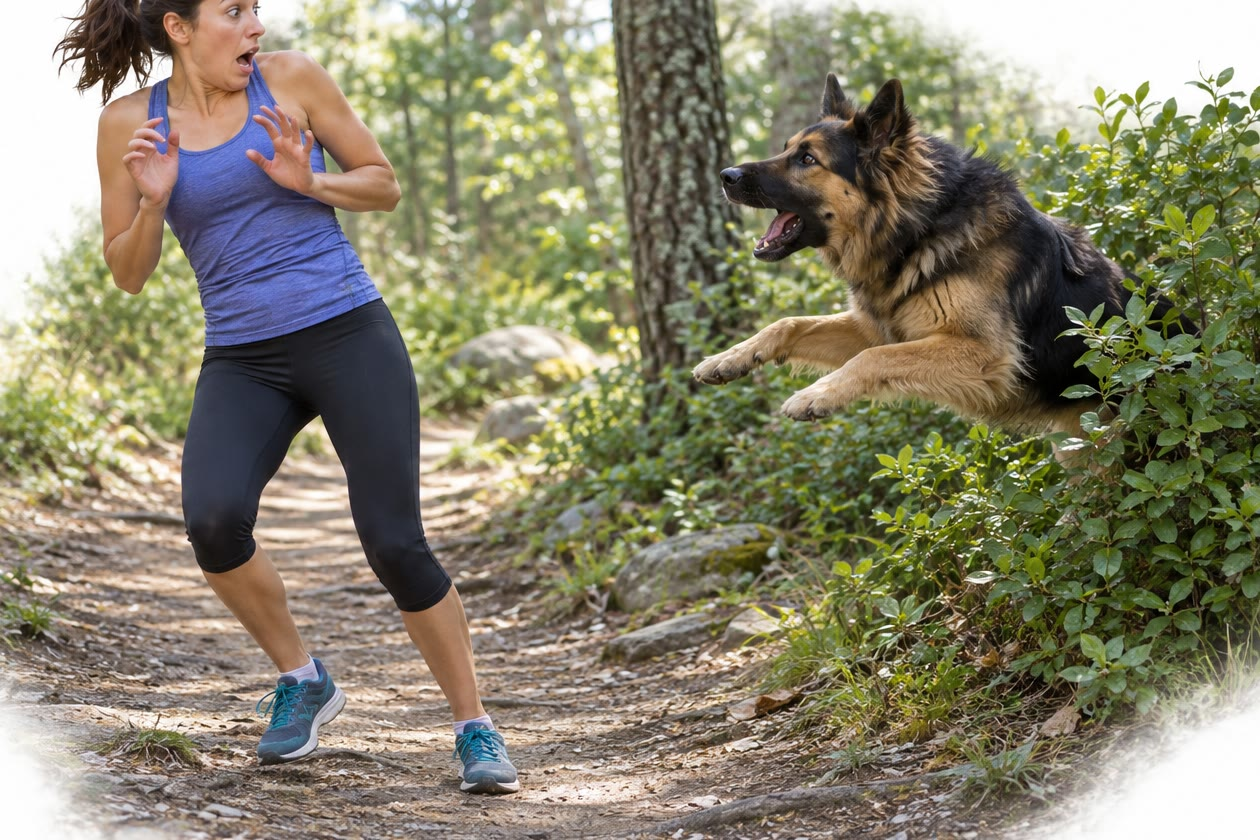
\includegraphics[width=0.6\linewidth]{images/book4/ai/b4-19-adrenaline-runner.jpg}

{\small A cascata em ação. Um susto libera adrenalina da medula
suprarrenal; em segundos, o \omterm{def:b2:heart:anatomy}{coração} dispara, o fígado despeja glicose e
as vias aéreas se dilatam --- um mensageiro, vários receptores, uma
amplificação de um milhão de vezes em cada célula.}
\end{omfigure}

\section{Os receptores internos}

\begin{proposition}[Os receptores nucleares]\label{prop:b2:cell-signalling:nuclear}
\index{receptor nuclear}\index{hormônio esteroide}
Os esteroides, a tiroxina, o ácido retinoico e a vitamina D se difundem
através da membrana e se ligam a receptores no citosol ou no núcleo que
são eles mesmos \emph{\omterm{prop:b2:cell-differentiation:transcriptional}{fatores de transcrição}}: o complexo
hormônio--receptor se liga a sequências específicas de DNA e liga ou
desliga seus genes-alvo. A resposta é lenta --- de minutos a horas para
produzir o mRNA e a proteína --- e duradoura: o cortisol induz as enzimas
da gliconeogênese durante horas, o estradiol constrói o revestimento
uterino ao longo de dias, a testosterona forma músculo ao longo de
semanas, a tiroxina fixa a taxa metabólica de todas as células. Alguns
esteroides também têm ações rápidas por meio de receptores de
superfície, e algumas vias de superfície também chegam ao núcleo (a
cascata das MAP quinases), de modo que a distinção não é absoluta; mas
a regra se mantém: um mensageiro lipossolúvel muda o que uma célula
\emph{é} mudando seus genes, enquanto um hidrossolúvel muda o que ela
\emph{faz} mudando suas enzimas.
\end{proposition}

\begin{omfigure}
\begin{tikzpicture}[every node/.style={font=\scriptsize}, >=stealth]
  \foreach \x/\t in {0/{hidrossolúveis: adrenalina, insulina, glucagon}, 7.4/{lipossolúveis: cortisol, estradiol, tiroxina}} \node[anchor=south, font=\scriptsize\bfseries] at (\x+2.6,3.4) {\t};
  % left: surface receptor
  \fill[omExo!30] (0,2.4) rectangle (5.2,2.8);
  \draw[thick, fill=omDef!40] (1.6,2.1) rectangle (2.3,3.1);
  \fill[omProp] (1.95,3.35) circle (0.1);
  \draw[->, thick] (1.95,2.1) -- (1.95,1.6) node[below, align=center] {segundos mensageiros,\\quinases: enzimas\\ativadas em segundos};
  \node[align=center] at (4.5,1.0) {muda o que\\a célula faz};
  % right: nuclear receptor
  \begin{scope}[xshift=7.4cm]
    \fill[omExo!30] (0,2.4) rectangle (5.2,2.8);
    \fill[omProp] (1.5,3.35) circle (0.1);
    \draw[->, omProp] (1.5,3.25) -- (1.5,1.9);
    \draw[thick, fill=omThm!20] (1.5,1.5) ellipse (0.72 and 0.3); \node at (1.5,1.5) {receptor};
    \draw[thick] (0.6,0.4) -- (4.6,0.4); \draw[thick] (0.6,0.25) -- (4.6,0.25); \node[below] at (2.6,0.2) {DNA: genes-alvo ligados ou desligados, horas};
    \draw[->, thick] (1.5,1.2) -- (2.4,0.5);
    \node[align=center] at (4.0,1.4) {muda o que\\a célula é};
  \end{scope}
\end{tikzpicture}

{\small Dois modelos. Um mensageiro hidrossolúvel age na superfície e
muda a atividade das enzimas em segundos; um lipossolúvel entra, se liga
a um receptor que é um \omterm{prop:b2:cell-differentiation:transcriptional}{fator de transcrição} e muda a expressão gênica
ao longo de horas.}
\end{omfigure}

\section{Um caso resolvido: insulina, glucagon e o valor de referência da glicose}

\begin{proposition}[Dois hormônios e um valor de referência]\label{prop:b2:cell-signalling:glucose}
\index{insulina}\index{glucagon}\index{glicemia}
A glicose do \omterm{def:b2:blood-circulation:blood}{sangue} é mantida perto de \qty{5}{mmol/L} (\qty{0.9}{g/L})
por dois \omterm{def:b2:cell-signalling:kinds}{hormônios} antagonistas das ilhotas pancreáticas. Após uma
refeição, a glicose em alta é percebida pelas células $\beta$ --- que a
metabolizam, fecham um canal de potássio à medida que seu ATP sobe, se
despolarizam, deixam entrar cálcio e liberam \emph{insulina} ---, e a
insulina, por meio de seu \omterm{prop:b2:cell-signalling:rtk}{receptor tirosina quinase}, faz os músculos e
o tecido adiposo captarem glicose (deslocando transportadores para suas
membranas), o fígado armazená-la como glicogênio e gordura, e todos os
tecidos pararem de queimar gordura. Entre as refeições, a glicose em
queda deixa as células $\alpha$ liberarem \emph{glucagon}, que, por meio
do AMPc no fígado, degrada o glicogênio e produz glicose nova a partir
de aminoácidos; a adrenalina faz o mesmo mais depressa nas emergências,
e o cortisol e o \omterm{def:b2:cell-signalling:kinds}{hormônio} do crescimento, ao longo de horas. Cada
\omterm{def:b2:cell-signalling:kinds}{hormônio} é liberado em proporção ao desvio que corrige: uma
retroalimentação negativa com dois efetores, um para cada sentido, e um
valor de referência defendido com precisão de um quinto. O encéfalo,
que queima \qty{120}{g} de glicose por dia e não armazena nada, é o
órgão que a alça protege; o diabetes tipo 1 é a perda das células
$\beta$, e seu curso sem tratamento --- glicose a
\qty{20}{mmol/L}, gordura queimada por falta de insulina, ácido no
\omterm{def:b2:blood-circulation:blood}{sangue} --- é o aspecto da alça com um dos braços removido.
\end{proposition}

\begin{omfigure}
\begin{tikzpicture}
\begin{axis}[
  width=0.82\linewidth, height=5.6cm,
  axis x line=bottom, axis y line=left,
  xmin=0, xmax=6, ymin=0, ymax=1.1,
  xlabel={horas após uma refeição}, ylabel={em relação ao pico},
  xlabel style={font=\small, at={(axis description cs:0.5,-0.12)}, anchor=north},
  ylabel style={font=\small},
  tick label style={font=\small}, xtick={0,1,2,3,4,5,6}, ytick={0,0.5,1},
  legend style={font=\scriptsize, at={(0.5,-0.28)}, anchor=north, draw=none, legend columns=3},
  clip=false,
]
\addplot[very thick, omDef, domain=0:6, samples=80] {0.55 + 0.45*exp(-((x-0.9)^2)/0.5) - 0.08*exp(-((x-4)^2)/2)};
\addlegendentry{glicemia (5 mmol/L em 0.55)}
\addplot[very thick, omThm, domain=0:6, samples=80] {0.15 + 0.85*exp(-((x-1.1)^2)/0.45)};
\addlegendentry{insulina}
\addplot[very thick, omProp, domain=0:6, samples=80] {0.75 - 0.5*exp(-((x-1.2)^2)/0.8) + 0.25*(1-exp(-x/5))*0.6};
\addlegendentry{glucagon}
\end{axis}
\end{tikzpicture}

{\small Glicose, insulina e glucagon após uma refeição. A insulina sobe
com a glicose e a faz baixar; à medida que a glicose cai em direção ao
valor de referência, o glucagon sobe para mantê-la ali.}
\end{omfigure}

\begin{example}[Velocidade, alcance e custo dos dois sistemas]\label{ex:b2:cell-signalling:compare}
A adrenalina no \omterm{def:b2:blood-circulation:blood}{sangue} chega a todas as células em cerca de um minuto
(o tempo de circulação) e age durante minutos; um impulso nervoso chega
a seu alvo em milissegundos e age durante milissegundos. Um \omterm{def:b2:cell-signalling:kinds}{hormônio}
custa quase nada por célula alcançada --- um nanomol espalhado pelo
corpo ---, mas não consegue se dirigir a uma única célula; um nervo se
dirige exatamente a uma célula, mas precisa construir e manter um fio
até ela. O corpo usa os dois: os nervos simpáticos do \cref{ch:b2:blood-pressure} agem
sobre o \omterm{def:b2:heart:anatomy}{coração} e as \omterm{def:b2:blood-circulation:vessels}{arteríolas} em um segundo, e a medula suprarrenal,
ela mesma um gânglio simpático modificado, os reforça despejando a mesma
molécula no \omterm{def:b2:blood-circulation:blood}{sangue} para o corpo inteiro. E, na sinapse, os dois modelos
se encontram, pois um \omterm{def:b2:cell-signalling:kinds}{neurotransmissor} é um mensageiro que age sobre um
receptor pelos mesmos mecanismos --- um canal que se abre, uma \omterm{prop:b2:cell-signalling:gpcr}{proteína
G} que se ativa ---, apenas através de vinte nanômetros em vez de um
metro.
\end{example}

\section{Exercícios}

\begin{exercise}[$\star$]\label{exo:b2:cell-signalling:1}
Classifique como endócrino, parácrino, autócrino ou sináptico, e como
hidrossolúvel ou lipossolúvel: a insulina, o cortisol, a acetilcolina
numa sinapse, a histamina numa ferida, o estradiol, a adrenalina da
suprarrenal, o óxido nítrico do endotélio.
\end{exercise}

\begin{exercise}[$\star$]\label{exo:b2:cell-signalling:2}
Liste as etapas que vão da adrenalina na membrana da célula hepática à
glicose no \omterm{def:b2:blood-circulation:blood}{sangue}, e cite o mecanismo de desligamento de cada etapa.
\end{exercise}

\begin{exercise}[$\star$]\label{exo:b2:cell-signalling:3}
Compare os receptores de superfície e os nucleares: o que se liga a
eles, onde estão, com que rapidez agem, o que mudam.
\end{exercise}

\begin{exercise}[$\star$]\label{exo:b2:cell-signalling:4}
Quais são os três \omterm{prop:b2:cell-signalling:gpcr}{segundos mensageiros} universais citados neste
capítulo, como cada um é elevado e como cada um é removido?
\end{exercise}

\begin{exercise}[$\star\star$]\label{exo:b2:cell-signalling:5}
Um receptor tem $K_d = \qty{2}{nmol/L}$. Calcule a ocupação a 0.2, 2,
20 e \qty{200}{nmol/L}. Uma célula dobra seu número de receptores: o
que muda, a ocupação ou o número de receptores ocupados?
\end{exercise}

\begin{exercise}[$\star\star$]\label{exo:b2:cell-signalling:6}
Uma cascata tem etapas com ganhos de 50, 200, 100 e 300. Calcule a
amplificação total. Se o \omterm{def:b2:cell-signalling:kinds}{hormônio} está a \qty{1}{nmol/L} e
\qty{1}{\%} dos receptores ($10^{4}$ por célula) está ocupado, quantas
moléculas de produto a célula produz por segundo, se o ganho de cada
etapa é por segundo?
\end{exercise}

\begin{exercise}[$\star\star$]\label{exo:b2:cell-signalling:7}
A toxina colérica trava a \omterm{prop:b2:cell-signalling:gpcr}{proteína G} estimuladora em seu estado ligado
ao GTP nas células intestinais. Explique, passo a passo, por que o
paciente perde litros de líquido por dia, e por que o efeito persiste
durante dias depois que as bactérias desaparecem.
\end{exercise}

\begin{exercise}[$\star\star$]\label{exo:b2:cell-signalling:8}
O cálcio citosólico sobe de \qty{0.1}{} a \qty{1}{\micro
mol/L} numa célula de \qty{2000}{\micro m^3} quando um canal se abre.
Quantos íons de cálcio entraram? Se um único canal aberto deixa passar
$10^{6}$ íons por segundo, quanto tempo um único canal levou, e por que
uma célula abre muitos canais ao mesmo tempo?
\end{exercise}

\begin{exercise}[$\star\star$]\label{exo:b2:cell-signalling:9}
A insulina e o glucagon agem ambos sobre o fígado, um por meio de uma
tirosina quinase e o outro por meio do AMPc. Explique como a célula
hepática integra os dois sinais, o que acontece com o glicogênio quando
ambos estão altos, e por que a razão entre eles importa mais do que
cada nível.
\end{exercise}

\begin{exercise}[$\star\star\star$]\label{exo:b2:cell-signalling:10}
A adrenalina eleva o AMPc numa célula hepática em \qty{5}{s} e a
produção de glicose em \qty{30}{s}; o cortisol eleva as enzimas
gliconeogênicas do fígado ao longo de \qty{4}{h}. Usando a difusão, a
transcrição (\qty{50}{} nucleotídeos por segundo num gene de
\qty{3000}{} nucleotídeos), a tradução (\qty{5}{} aminoácidos por
segundo numa proteína de \num{500} resíduos) e a necessidade de
acumular milhares de moléculas de enzima, explique as duas escalas de
tempo.
\end{exercise}

\begin{exercise}[$\star\star\star$]\label{exo:b2:cell-signalling:11}
Uma \omterm{def:b2:genome-diversification:mutation}{mutação} faz um \omterm{prop:b2:cell-signalling:rtk}{receptor tirosina quinase} de fator de crescimento se
dimerizar, e portanto sinalizar, sem seu ligante. Preveja o
comportamento da célula, explique por que essa é uma etapa comum no
câncer, e diga o que faria um fármaco que bloqueia o sítio de ATP da
quinase.
\end{exercise}

\begin{exercise}[$\star\star\star$]\label{exo:b2:cell-signalling:12}
``O sistema endócrino transmite para todos; o sistema nervoso liga por
fios.'' Discuta os dois modelos quanto à velocidade, ao alcance, à
especificidade e ao custo, e diga onde cada um é indispensável e onde o
corpo usa ambos para a mesma mensagem.
\end{exercise}

\section{Problema: Um hormônio do sangue ao gene}

\begin{problem}[{Problema de fim de semana --- a adrenalina acompanhada
da glândula suprarrenal até a glicose de uma célula hepática, com sua
concentração, a ocupação dos receptores, o ganho da cascata e o tempo
calculados, depois o cortisol acompanhado até um gene, e a alça da
glicose analisada, até a ocupação, a amplificação e o tempo que cada
hormônio leva}]
\label{pb:b2:cell-signalling:1}
Dados: a medula suprarrenal libera \qty{1}{nmol} de adrenalina em
\qty{5}{L} de \omterm{def:b2:blood-circulation:blood}{sangue} num susto; o $K_d$ da adrenalina no receptor
hepático é \qty{1}{nmol/L}; uma célula hepática (\qty{5000}{\micro m^3})
tem $2\times 10^{4}$ receptores. Ganhos da cascata por segundo de
ativação: receptor $\to$ \omterm{prop:b2:cell-signalling:gpcr}{proteína G} 20, \omterm{prop:b2:cell-signalling:gpcr}{proteína G} $\to$ AMPc 100 (o
número de ciclos da ciclase durante os 3 segundos de vida da \omterm{prop:b2:cell-signalling:gpcr}{proteína
G}), AMPc $\to$ quinase A 1 (estequiométrico), quinase A $\to$
fosforilase quinase 50, $\to$ fosforilase 50, $\to$ glicose 1000. O
fígado contém \qty{100}{g} de glicogênio. Cortisol: transcrição a
\qty{50}{} nucleotídeos por segundo num gene de \qty{4000}{}
nucleotídeos, tradução a \qty{5}{} resíduos por segundo numa enzima de
\num{600} resíduos, \num{20} ribossomos por mRNA, \num{100} mRNAs
produzidos por hora, um efeito que exige $10^{5}$ moléculas de enzima.

\medskip
\noindent\textbf{Parte I --- O \omterm{def:b2:cell-signalling:kinds}{hormônio} chega.}
\begin{enumerate}
  \item Calcule a concentração plasmática de adrenalina após a
        liberação, desprezando sua remoção.
  \item Calcule a \omterm{thm:b2:cell-signalling:occupancy}{ocupação dos receptores} e o número de receptores
        ocupados por célula hepática.
  \item A adrenalina é removida com uma meia-vida de \qty{2}{min}. Qual
        é sua concentração, e a ocupação, após \qty{6}{min}?
  \item Quanto tempo a adrenalina leva para ir da suprarrenal ao fígado,
        dado um tempo de circulação de cerca de um minuto? Por que o
        nervo simpático do fígado age mais depressa?
  \item Uma célula com $2\times 10^{5}$ receptores e o mesmo $K_d$: o
        que muda?
  \item Por que o $K_d$ está ajustado à concentração circulante --- o
        que faria um receptor com $K_d = \qty{1}{\micro mol/L}$ diante de
        um \omterm{def:b2:cell-signalling:kinds}{hormônio} nanomolar?
\end{enumerate}

\medskip
\noindent\textbf{Parte II --- A cascata.}
\begin{enumerate}[resume]
  \item Calcule o ganho total, de um receptor ocupado até as moléculas
        de glicose por segundo.
  \item Calcule as moléculas de AMPc que a célula produz no primeiro
        segundo e a concentração que elas atingem em seu volume.
  \item Calcule a produção de glicose de uma célula hepática por segundo
        com a ocupação da questão 2, e por minuto.
  \item O fígado tem $2\times 10^{11}$ células. Calcule a produção que os
        ganhos preveem, em gramas por minuto, e compare com os
        \qty{5}{g/min} observados de fato. O que limita a produção real?
  \item Quanto tempo os \qty{100}{g} de glicogênio durariam nesse ritmo?
        Por que eles não se esgotam num susto?
  \item Cite o mecanismo de desligamento de cada etapa amplificadora e
        diga qual age mais depressa.
  \item Há um inibidor da fosfodiesterase (a cafeína) presente. Preveja
        o efeito sobre a cascata e sobre a produção de glicose.
\end{enumerate}

\medskip
\noindent\textbf{Parte III --- Do cortisol ao gene.}
\begin{enumerate}[resume]
  \item Calcule o tempo para transcrever um mRNA.
  \item Calcule o tempo para traduzir uma molécula de enzima e o número
        de moléculas de enzima por mRNA por hora (cada mRNA vivendo uma
        hora, com os ribossomos começando um após o outro).
  \item Calcule as moléculas de enzima produzidas por hora a partir dos
        \num{100} mRNAs e o tempo para chegar a $10^{5}$.
  \item Acrescente o tempo para o cortisol entrar, se ligar e chegar ao
        DNA (minutos) e explique as \qty{4}{h} observadas.
  \item Por que o corpo não usaria uma cascata como a da adrenalina para
        a função do cortisol, e por que não usaria o mecanismo do cortisol
        para um susto?
  \item O cortisol também aumenta o número de receptores de adrenalina
        nas células hepáticas. Explique como um \omterm{def:b2:cell-signalling:kinds}{hormônio} lento pode
        amplificar um rápido, e o que isso faz com a curva de ocupação do
        \omterm{def:b2:cell-signalling:kinds}{hormônio} rápido.
\end{enumerate}

\medskip
\noindent\textbf{Parte IV --- A alça.}
\begin{enumerate}[resume]
  \item Após uma refeição, a glicose sobe de 5 para \qty{8}{mmol/L}.
        Descreva a resposta da célula $\beta$, da glicose à liberação de
        insulina, indicando o acoplamento.
  \item A insulina age por meio de uma tirosina quinase; o glucagon, por
        meio do AMPc. Explique por que uma única célula pode obedecer aos
        dois e como as enzimas do glicogênio do fígado são reguladas pela
        razão entre eles.
  \item Um paciente não tem células $\beta$. Preveja a glicose em jejum
        e após as refeições, e explique por que a gordura é queimada e
        surge ácido.
  \item A insulina injetada não tem retroalimentação. Explique o perigo
        de uma corrida excepcionalmente longa com a dose habitual.
  \item Compare a alça da glicose com o \omterm{def:b2:blood-pressure:baroreflex}{barorreflexo} do \cref{ch:b2:blood-pressure}:
        sensor, efetores, ganho, velocidade.
  \item Enuncie o resultado: a ocupação da adrenalina após a liberação,
        o ganho da cascata, a produção de glicose do fígado e o tempo que
        o cortisol leva.
\end{enumerate}
\end{problem}
